% Options for packages loaded elsewhere
\PassOptionsToPackage{unicode}{hyperref}
\PassOptionsToPackage{hyphens}{url}
%
\documentclass[
]{article}
\usepackage{amsmath,amssymb}
\usepackage{lmodern}
\usepackage{iftex}
\ifPDFTeX
  \usepackage[T1]{fontenc}
  \usepackage[utf8]{inputenc}
  \usepackage{textcomp} % provide euro and other symbols
\else % if luatex or xetex
  \usepackage{unicode-math}
  \defaultfontfeatures{Scale=MatchLowercase}
  \defaultfontfeatures[\rmfamily]{Ligatures=TeX,Scale=1}
\fi
% Use upquote if available, for straight quotes in verbatim environments
\IfFileExists{upquote.sty}{\usepackage{upquote}}{}
\IfFileExists{microtype.sty}{% use microtype if available
  \usepackage[]{microtype}
  \UseMicrotypeSet[protrusion]{basicmath} % disable protrusion for tt fonts
}{}
\makeatletter
\@ifundefined{KOMAClassName}{% if non-KOMA class
  \IfFileExists{parskip.sty}{%
    \usepackage{parskip}
  }{% else
    \setlength{\parindent}{0pt}
    \setlength{\parskip}{6pt plus 2pt minus 1pt}}
}{% if KOMA class
  \KOMAoptions{parskip=half}}
\makeatother
\usepackage{xcolor}
\IfFileExists{xurl.sty}{\usepackage{xurl}}{} % add URL line breaks if available
\IfFileExists{bookmark.sty}{\usepackage{bookmark}}{\usepackage{hyperref}}
\hypersetup{
  hidelinks,
  pdfcreator={LaTeX via pandoc}}
\urlstyle{same} % disable monospaced font for URLs
\usepackage{listings}
\newcommand{\passthrough}[1]{#1}
\lstset{defaultdialect=[5.3]Lua}
\lstset{defaultdialect=[x86masm]Assembler}
\usepackage{graphicx}
\makeatletter
\def\maxwidth{\ifdim\Gin@nat@width>\linewidth\linewidth\else\Gin@nat@width\fi}
\def\maxheight{\ifdim\Gin@nat@height>\textheight\textheight\else\Gin@nat@height\fi}
\makeatother
% Scale images if necessary, so that they will not overflow the page
% margins by default, and it is still possible to overwrite the defaults
% using explicit options in \includegraphics[width, height, ...]{}
\setkeys{Gin}{width=\maxwidth,height=\maxheight,keepaspectratio}
% Set default figure placement to htbp
\makeatletter
\def\fps@figure{htbp}
\makeatother
\setlength{\emergencystretch}{3em} % prevent overfull lines
\providecommand{\tightlist}{%
  \setlength{\itemsep}{0pt}\setlength{\parskip}{0pt}}
\setcounter{secnumdepth}{-\maxdimen} % remove section numbering
\ifLuaTeX
  \usepackage{selnolig}  % disable illegal ligatures
\fi

\author{}
\date{}

\begin{document}

\begin{lstlisting}[language=Python]
import numpy as np
import matplotlib.pyplot as plt
import pandas as pd
from numpy import random
import sklearn
\end{lstlisting}

\textbf{STEP 1: Load the iris flower dataset}

\begin{lstlisting}[language=Python]
from sklearn.datasets import load_iris
iris = load_iris()

X = iris.data    # X is 2d array, where row=samples, column=features
y = iris.target  # y is 1d array, representing class label for all samples
\end{lstlisting}

\begin{lstlisting}[language=Python]
print(X.shape)
print(y.shape)
print(iris.feature_names)
print("Target names:", iris.target_names)
\end{lstlisting}

\begin{lstlisting}
(150, 4)
(150,)
['sepal length (cm)', 'sepal width (cm)', 'petal length (cm)', 'petal width (cm)']
Target names: ['setosa' 'versicolor' 'virginica']
\end{lstlisting}

\begin{lstlisting}[language=Python]
print(X)
\end{lstlisting}

\begin{lstlisting}
[[5.1 3.5 1.4 0.2]
 [4.9 3.  1.4 0.2]
 [4.7 3.2 1.3 0.2]
 [4.6 3.1 1.5 0.2]
 [5.  3.6 1.4 0.2]
 [5.4 3.9 1.7 0.4]
 [4.6 3.4 1.4 0.3]
 [5.  3.4 1.5 0.2]
 [4.4 2.9 1.4 0.2]
 [4.9 3.1 1.5 0.1]
 [5.4 3.7 1.5 0.2]
 [4.8 3.4 1.6 0.2]
 [4.8 3.  1.4 0.1]
 [4.3 3.  1.1 0.1]
 [5.8 4.  1.2 0.2]
 [5.7 4.4 1.5 0.4]
 [5.4 3.9 1.3 0.4]
 [5.1 3.5 1.4 0.3]
 [5.7 3.8 1.7 0.3]
 [5.1 3.8 1.5 0.3]
 [5.4 3.4 1.7 0.2]
 [5.1 3.7 1.5 0.4]
 [4.6 3.6 1.  0.2]
 [5.1 3.3 1.7 0.5]
 [4.8 3.4 1.9 0.2]
 [5.  3.  1.6 0.2]
 [5.  3.4 1.6 0.4]
 [5.2 3.5 1.5 0.2]
 [5.2 3.4 1.4 0.2]
 [4.7 3.2 1.6 0.2]
 [4.8 3.1 1.6 0.2]
 [5.4 3.4 1.5 0.4]
 [5.2 4.1 1.5 0.1]
 [5.5 4.2 1.4 0.2]
 [4.9 3.1 1.5 0.2]
 [5.  3.2 1.2 0.2]
 [5.5 3.5 1.3 0.2]
 [4.9 3.6 1.4 0.1]
 [4.4 3.  1.3 0.2]
 [5.1 3.4 1.5 0.2]
 [5.  3.5 1.3 0.3]
 [4.5 2.3 1.3 0.3]
 [4.4 3.2 1.3 0.2]
 [5.  3.5 1.6 0.6]
 [5.1 3.8 1.9 0.4]
 [4.8 3.  1.4 0.3]
 [5.1 3.8 1.6 0.2]
 [4.6 3.2 1.4 0.2]
 [5.3 3.7 1.5 0.2]
 [5.  3.3 1.4 0.2]
 [7.  3.2 4.7 1.4]
 [6.4 3.2 4.5 1.5]
 [6.9 3.1 4.9 1.5]
 [5.5 2.3 4.  1.3]
 [6.5 2.8 4.6 1.5]
 [5.7 2.8 4.5 1.3]
 [6.3 3.3 4.7 1.6]
 [4.9 2.4 3.3 1. ]
 [6.6 2.9 4.6 1.3]
 [5.2 2.7 3.9 1.4]
 [5.  2.  3.5 1. ]
 [5.9 3.  4.2 1.5]
 [6.  2.2 4.  1. ]
 [6.1 2.9 4.7 1.4]
 [5.6 2.9 3.6 1.3]
 [6.7 3.1 4.4 1.4]
 [5.6 3.  4.5 1.5]
 [5.8 2.7 4.1 1. ]
 [6.2 2.2 4.5 1.5]
 [5.6 2.5 3.9 1.1]
 [5.9 3.2 4.8 1.8]
 [6.1 2.8 4.  1.3]
 [6.3 2.5 4.9 1.5]
 [6.1 2.8 4.7 1.2]
 [6.4 2.9 4.3 1.3]
 [6.6 3.  4.4 1.4]
 [6.8 2.8 4.8 1.4]
 [6.7 3.  5.  1.7]
 [6.  2.9 4.5 1.5]
 [5.7 2.6 3.5 1. ]
 [5.5 2.4 3.8 1.1]
 [5.5 2.4 3.7 1. ]
 [5.8 2.7 3.9 1.2]
 [6.  2.7 5.1 1.6]
 [5.4 3.  4.5 1.5]
 [6.  3.4 4.5 1.6]
 [6.7 3.1 4.7 1.5]
 [6.3 2.3 4.4 1.3]
 [5.6 3.  4.1 1.3]
 [5.5 2.5 4.  1.3]
 [5.5 2.6 4.4 1.2]
 [6.1 3.  4.6 1.4]
 [5.8 2.6 4.  1.2]
 [5.  2.3 3.3 1. ]
 [5.6 2.7 4.2 1.3]
 [5.7 3.  4.2 1.2]
 [5.7 2.9 4.2 1.3]
 [6.2 2.9 4.3 1.3]
 [5.1 2.5 3.  1.1]
 [5.7 2.8 4.1 1.3]
 [6.3 3.3 6.  2.5]
 [5.8 2.7 5.1 1.9]
 [7.1 3.  5.9 2.1]
 [6.3 2.9 5.6 1.8]
 [6.5 3.  5.8 2.2]
 [7.6 3.  6.6 2.1]
 [4.9 2.5 4.5 1.7]
 [7.3 2.9 6.3 1.8]
 [6.7 2.5 5.8 1.8]
 [7.2 3.6 6.1 2.5]
 [6.5 3.2 5.1 2. ]
 [6.4 2.7 5.3 1.9]
 [6.8 3.  5.5 2.1]
 [5.7 2.5 5.  2. ]
 [5.8 2.8 5.1 2.4]
 [6.4 3.2 5.3 2.3]
 [6.5 3.  5.5 1.8]
 [7.7 3.8 6.7 2.2]
 [7.7 2.6 6.9 2.3]
 [6.  2.2 5.  1.5]
 [6.9 3.2 5.7 2.3]
 [5.6 2.8 4.9 2. ]
 [7.7 2.8 6.7 2. ]
 [6.3 2.7 4.9 1.8]
 [6.7 3.3 5.7 2.1]
 [7.2 3.2 6.  1.8]
 [6.2 2.8 4.8 1.8]
 [6.1 3.  4.9 1.8]
 [6.4 2.8 5.6 2.1]
 [7.2 3.  5.8 1.6]
 [7.4 2.8 6.1 1.9]
 [7.9 3.8 6.4 2. ]
 [6.4 2.8 5.6 2.2]
 [6.3 2.8 5.1 1.5]
 [6.1 2.6 5.6 1.4]
 [7.7 3.  6.1 2.3]
 [6.3 3.4 5.6 2.4]
 [6.4 3.1 5.5 1.8]
 [6.  3.  4.8 1.8]
 [6.9 3.1 5.4 2.1]
 [6.7 3.1 5.6 2.4]
 [6.9 3.1 5.1 2.3]
 [5.8 2.7 5.1 1.9]
 [6.8 3.2 5.9 2.3]
 [6.7 3.3 5.7 2.5]
 [6.7 3.  5.2 2.3]
 [6.3 2.5 5.  1.9]
 [6.5 3.  5.2 2. ]
 [6.2 3.4 5.4 2.3]
 [5.9 3.  5.1 1.8]]
\end{lstlisting}

\textbf{STEP 2: Create a dataframe and see the data statistics}

\begin{lstlisting}[language=Python]
# assign meaningful columns(feature_names) to feature values for 150 samples(iris.data) in the dataframe.
df = pd.DataFrame(data=iris.data,columns=iris.feature_names)
# add a new target column.
df['target']=iris.target

df.head(2)   # view 1st 2 data, both are setosa(numbering starts from 0)
\end{lstlisting}

sepal length (cm)

sepal width (cm)

petal length (cm)

petal width (cm)

target

0

5.1

3.5

1.4

0.2

0

1

4.9

3.0

1.4

0.2

0

\begin{lstlisting}[language=Python]
#view 49th to 52nd dataset to see 2 classes(setosa and vesicolor)
subset = df.iloc[48:52]
print(subset)
\end{lstlisting}

\begin{lstlisting}
    sepal length (cm)  sepal width (cm)  petal length (cm)  petal width (cm)  \
48                5.3               3.7                1.5               0.2   
49                5.0               3.3                1.4               0.2   
50                7.0               3.2                4.7               1.4   
51                6.4               3.2                4.5               1.5   

    target  
48       0  
49       0  
50       1  
51       1  
\end{lstlisting}

\begin{lstlisting}[language=Python]
# statistics computed for each column
summary_stats = df.describe()
print(summary_stats)
\end{lstlisting}

\begin{lstlisting}
       sepal length (cm)  sepal width (cm)  petal length (cm)  \
count         150.000000        150.000000         150.000000   
mean            5.843333          3.057333           3.758000   
std             0.828066          0.435866           1.765298   
min             4.300000          2.000000           1.000000   
25%             5.100000          2.800000           1.600000   
50%             5.800000          3.000000           4.350000   
75%             6.400000          3.300000           5.100000   
max             7.900000          4.400000           6.900000   

       petal width (cm)      target  
count        150.000000  150.000000  
mean           1.199333    1.000000  
std            0.762238    0.819232  
min            0.100000    0.000000  
25%            0.300000    0.000000  
50%            1.300000    1.000000  
75%            1.800000    2.000000  
max            2.500000    2.000000  
\end{lstlisting}

\begin{lstlisting}[language=Python]
# data visualization, box plot for each feature
df.plot(kind='box', figsize=(10, 6))
plt.title('Box Plot of Iris Dataset')
plt.text(1.5, 8, "'THA076BCT026','THA076BCT027','THA076BCT041'", fontsize=8,color='red')


plt.savefig('Box Plot of Iris Dataset', bbox_inches='tight')
plt.show()
\end{lstlisting}

\begin{figure}
\centering
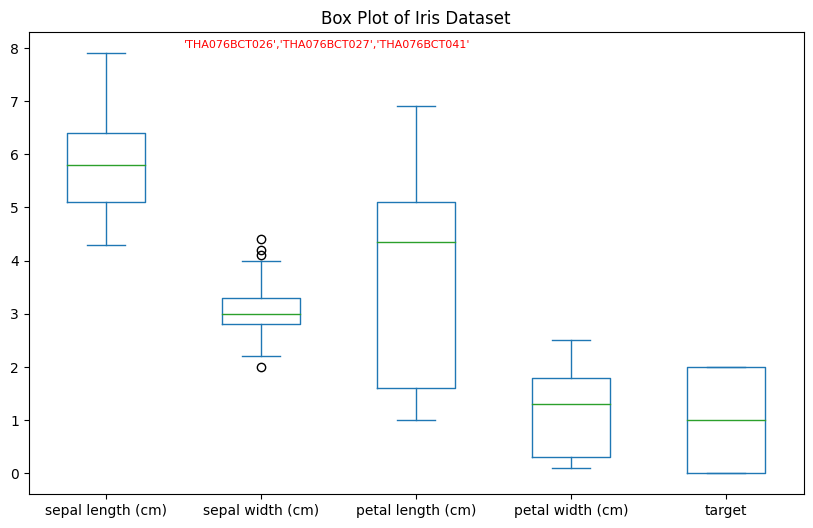
\includegraphics{PCA on IRIS_files/PCA on IRIS_9_0.png}
\caption{png}
\end{figure}

\begin{lstlisting}[language=Python]
import seaborn as sns
# plt.figure(figsize=(12, 8))
# sns.pairplot(df, hue = 'target')
# plt.title('Attribute Correlation Heatmap')
# plt.text(0.5, 8, "'THA076BCT026','THA076BCT027','THA076BCT041'", fontsize=8,color='red')
# plt.savefig('./plots/pair Plot', bbox_inches='tight')
# plt.show()
# Set the size of the figure
plt.figure(figsize=(12, 7))
df['target'] = df['target'].replace({0: 'Setosa', 1: 'Versicolor', 2: 'Virginica'})
# Create a pair plot with hue based on the 'target' column in the dataframe
g=sns.pairplot(df, hue='target',plot_kws={'legend': False})
g._legend.set_title('')
# target_labels = ['Setosa', 'Versicolor', 'Virginica']
# # Set the title of the plot
plt.suptitle('Attribute Correlation Pair Plot', fontsize=16, y=0.98)



# Set the style and color of the text box
textbox_props = dict(boxstyle='round', facecolor='white', edgecolor='gray', alpha=0.8)

# Add a text box with the highlighted feature names
plt.text(0.1, 8, "THA076BCT026\nTHA076BCT027\nTHA076BCT041", fontsize=10, color='red', ha='center', bbox=textbox_props)
legend_elements = [plt.Line2D([0], [0], marker='o', color='w', label='Setosa', markerfacecolor='royalblue', markersize=8),
                   plt.Line2D([0], [0], marker='o', color='w', label='Versicolor', markerfacecolor='g', markersize=8),
                   plt.Line2D([0], [0], marker='o', color='w', label='Virginica', markerfacecolor='orange', markersize=8)]

# Add the legend to the plot
plt.legend(handles=legend_elements, title='target')

# Adjust the spacing between subplots
plt.subplots_adjust(top=0.9)

# Set custom tick labels for the legend
# plt.gca().get_legend().remove()
# plt.legend(title='Target', labels=target_labels)
# Save the plot to a file
plt.savefig('./plots/pair_plot.png', bbox_inches='tight')


# Display the plot
plt.show()
\end{lstlisting}

\begin{lstlisting}
<Figure size 1200x700 with 0 Axes>
\end{lstlisting}

\begin{figure}
\centering
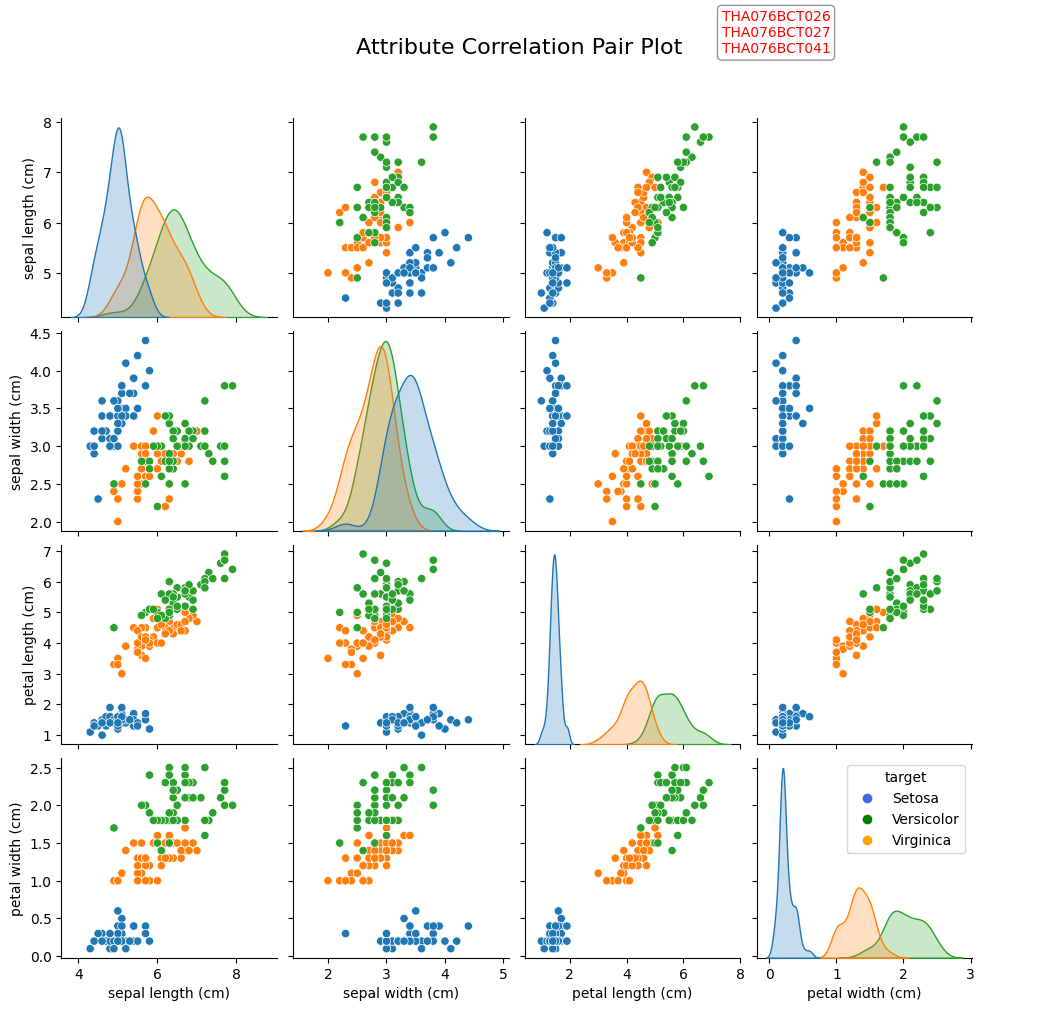
\includegraphics{PCA on IRIS_files/PCA on IRIS_10_1.png}
\caption{png}
\end{figure}

\begin{lstlisting}[language=Python]
# Visualization of data points based on the target class (purple=setosa,green=Versicolour,yellow=Virginica )
df['target']=iris.target
plt.figure(figsize=(10, 6))
plt.scatter(df['sepal length (cm)'], df['sepal width (cm)'], c=df['target'], label='Sepal')
plt.scatter(df['petal length (cm)'], df['petal width (cm)'], c=df['target'], marker='x', label='Petal')
plt.xlabel('Length (cm)')
plt.ylabel('Width (cm)')
plt.title('Scatter Plot of Sepal and Petal Features')
plt.colorbar(label='Species')
plt.text(1, 4.3, "'THA076BCT026','THA076BCT027','THA076BCT041'", fontsize=8,color='red')
plt.legend()
plt.savefig('./plots/Sepal and Petal Features', bbox_inches='tight')
plt.show()
\end{lstlisting}

\begin{figure}
\centering
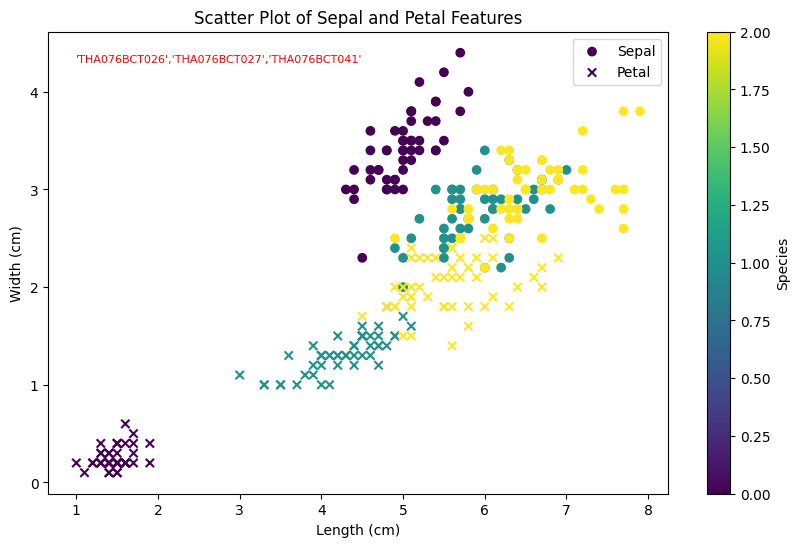
\includegraphics{PCA on IRIS_files/PCA on IRIS_11_0.png}
\caption{png}
\end{figure}

\textbf{STEP 3: Data preprocessing}

\begin{lstlisting}[language=Python]
# Handling missing values:
# df.isna() returns a boolean, where True means missing values(NaN) and .sum() sums the values along each column
missing_values = df.isna().sum()
print("Columns with missing values:")
print(missing_values[missing_values > 0])
\end{lstlisting}

\begin{lstlisting}
Columns with missing values:
Series([], dtype: int64)
\end{lstlisting}

\begin{lstlisting}[language=Python]
# Standardizing to eliminate the chance of PCA being influenced by magnitude of some features' values.
from sklearn.preprocessing import StandardScaler
scaler = StandardScaler()
X = df.iloc[:,1:].values
df_scaled = pd.DataFrame(scaler.fit_transform(df), columns=df.columns)
\end{lstlisting}

\begin{lstlisting}[language=Python]
# IMPORTANT STEP!
# Create new input and output after preprocessing X and y.
X_train = df_scaled.drop('target', axis=1).values
y_train = df['target']
print("shape of new input X",X_train.shape)
print("shape of new output Y",y_train.shape)
\end{lstlisting}

\begin{lstlisting}
shape of new input X (150, 4)
shape of new output Y (150,)
\end{lstlisting}

\begin{lstlisting}[language=Python]
print(X_train)
print(y_train)
\end{lstlisting}

\begin{lstlisting}
[[-9.00681170e-01  1.01900435e+00 -1.34022653e+00 -1.31544430e+00]
 [-1.14301691e+00 -1.31979479e-01 -1.34022653e+00 -1.31544430e+00]
 [-1.38535265e+00  3.28414053e-01 -1.39706395e+00 -1.31544430e+00]
 [-1.50652052e+00  9.82172869e-02 -1.28338910e+00 -1.31544430e+00]
 [-1.02184904e+00  1.24920112e+00 -1.34022653e+00 -1.31544430e+00]
 [-5.37177559e-01  1.93979142e+00 -1.16971425e+00 -1.05217993e+00]
 [-1.50652052e+00  7.88807586e-01 -1.34022653e+00 -1.18381211e+00]
 [-1.02184904e+00  7.88807586e-01 -1.28338910e+00 -1.31544430e+00]
 [-1.74885626e+00 -3.62176246e-01 -1.34022653e+00 -1.31544430e+00]
 [-1.14301691e+00  9.82172869e-02 -1.28338910e+00 -1.44707648e+00]
 [-5.37177559e-01  1.47939788e+00 -1.28338910e+00 -1.31544430e+00]
 [-1.26418478e+00  7.88807586e-01 -1.22655167e+00 -1.31544430e+00]
 [-1.26418478e+00 -1.31979479e-01 -1.34022653e+00 -1.44707648e+00]
 [-1.87002413e+00 -1.31979479e-01 -1.51073881e+00 -1.44707648e+00]
 [-5.25060772e-02  2.16998818e+00 -1.45390138e+00 -1.31544430e+00]
 [-1.73673948e-01  3.09077525e+00 -1.28338910e+00 -1.05217993e+00]
 [-5.37177559e-01  1.93979142e+00 -1.39706395e+00 -1.05217993e+00]
 [-9.00681170e-01  1.01900435e+00 -1.34022653e+00 -1.18381211e+00]
 [-1.73673948e-01  1.70959465e+00 -1.16971425e+00 -1.18381211e+00]
 [-9.00681170e-01  1.70959465e+00 -1.28338910e+00 -1.18381211e+00]
 [-5.37177559e-01  7.88807586e-01 -1.16971425e+00 -1.31544430e+00]
 [-9.00681170e-01  1.47939788e+00 -1.28338910e+00 -1.05217993e+00]
 [-1.50652052e+00  1.24920112e+00 -1.56757623e+00 -1.31544430e+00]
 [-9.00681170e-01  5.58610819e-01 -1.16971425e+00 -9.20547742e-01]
 [-1.26418478e+00  7.88807586e-01 -1.05603939e+00 -1.31544430e+00]
 [-1.02184904e+00 -1.31979479e-01 -1.22655167e+00 -1.31544430e+00]
 [-1.02184904e+00  7.88807586e-01 -1.22655167e+00 -1.05217993e+00]
 [-7.79513300e-01  1.01900435e+00 -1.28338910e+00 -1.31544430e+00]
 [-7.79513300e-01  7.88807586e-01 -1.34022653e+00 -1.31544430e+00]
 [-1.38535265e+00  3.28414053e-01 -1.22655167e+00 -1.31544430e+00]
 [-1.26418478e+00  9.82172869e-02 -1.22655167e+00 -1.31544430e+00]
 [-5.37177559e-01  7.88807586e-01 -1.28338910e+00 -1.05217993e+00]
 [-7.79513300e-01  2.40018495e+00 -1.28338910e+00 -1.44707648e+00]
 [-4.16009689e-01  2.63038172e+00 -1.34022653e+00 -1.31544430e+00]
 [-1.14301691e+00  9.82172869e-02 -1.28338910e+00 -1.31544430e+00]
 [-1.02184904e+00  3.28414053e-01 -1.45390138e+00 -1.31544430e+00]
 [-4.16009689e-01  1.01900435e+00 -1.39706395e+00 -1.31544430e+00]
 [-1.14301691e+00  1.24920112e+00 -1.34022653e+00 -1.44707648e+00]
 [-1.74885626e+00 -1.31979479e-01 -1.39706395e+00 -1.31544430e+00]
 [-9.00681170e-01  7.88807586e-01 -1.28338910e+00 -1.31544430e+00]
 [-1.02184904e+00  1.01900435e+00 -1.39706395e+00 -1.18381211e+00]
 [-1.62768839e+00 -1.74335684e+00 -1.39706395e+00 -1.18381211e+00]
 [-1.74885626e+00  3.28414053e-01 -1.39706395e+00 -1.31544430e+00]
 [-1.02184904e+00  1.01900435e+00 -1.22655167e+00 -7.88915558e-01]
 [-9.00681170e-01  1.70959465e+00 -1.05603939e+00 -1.05217993e+00]
 [-1.26418478e+00 -1.31979479e-01 -1.34022653e+00 -1.18381211e+00]
 [-9.00681170e-01  1.70959465e+00 -1.22655167e+00 -1.31544430e+00]
 [-1.50652052e+00  3.28414053e-01 -1.34022653e+00 -1.31544430e+00]
 [-6.58345429e-01  1.47939788e+00 -1.28338910e+00 -1.31544430e+00]
 [-1.02184904e+00  5.58610819e-01 -1.34022653e+00 -1.31544430e+00]
 [ 1.40150837e+00  3.28414053e-01  5.35408562e-01  2.64141916e-01]
 [ 6.74501145e-01  3.28414053e-01  4.21733708e-01  3.95774101e-01]
 [ 1.28034050e+00  9.82172869e-02  6.49083415e-01  3.95774101e-01]
 [-4.16009689e-01 -1.74335684e+00  1.37546573e-01  1.32509732e-01]
 [ 7.95669016e-01 -5.92373012e-01  4.78571135e-01  3.95774101e-01]
 [-1.73673948e-01 -5.92373012e-01  4.21733708e-01  1.32509732e-01]
 [ 5.53333275e-01  5.58610819e-01  5.35408562e-01  5.27406285e-01]
 [-1.14301691e+00 -1.51316008e+00 -2.60315415e-01 -2.62386821e-01]
 [ 9.16836886e-01 -3.62176246e-01  4.78571135e-01  1.32509732e-01]
 [-7.79513300e-01 -8.22569778e-01  8.07091462e-02  2.64141916e-01]
 [-1.02184904e+00 -2.43394714e+00 -1.46640561e-01 -2.62386821e-01]
 [ 6.86617933e-02 -1.31979479e-01  2.51221427e-01  3.95774101e-01]
 [ 1.89829664e-01 -1.97355361e+00  1.37546573e-01 -2.62386821e-01]
 [ 3.10997534e-01 -3.62176246e-01  5.35408562e-01  2.64141916e-01]
 [-2.94841818e-01 -3.62176246e-01 -8.98031345e-02  1.32509732e-01]
 [ 1.03800476e+00  9.82172869e-02  3.64896281e-01  2.64141916e-01]
 [-2.94841818e-01 -1.31979479e-01  4.21733708e-01  3.95774101e-01]
 [-5.25060772e-02 -8.22569778e-01  1.94384000e-01 -2.62386821e-01]
 [ 4.32165405e-01 -1.97355361e+00  4.21733708e-01  3.95774101e-01]
 [-2.94841818e-01 -1.28296331e+00  8.07091462e-02 -1.30754636e-01]
 [ 6.86617933e-02  3.28414053e-01  5.92245988e-01  7.90670654e-01]
 [ 3.10997534e-01 -5.92373012e-01  1.37546573e-01  1.32509732e-01]
 [ 5.53333275e-01 -1.28296331e+00  6.49083415e-01  3.95774101e-01]
 [ 3.10997534e-01 -5.92373012e-01  5.35408562e-01  8.77547895e-04]
 [ 6.74501145e-01 -3.62176246e-01  3.08058854e-01  1.32509732e-01]
 [ 9.16836886e-01 -1.31979479e-01  3.64896281e-01  2.64141916e-01]
 [ 1.15917263e+00 -5.92373012e-01  5.92245988e-01  2.64141916e-01]
 [ 1.03800476e+00 -1.31979479e-01  7.05920842e-01  6.59038469e-01]
 [ 1.89829664e-01 -3.62176246e-01  4.21733708e-01  3.95774101e-01]
 [-1.73673948e-01 -1.05276654e+00 -1.46640561e-01 -2.62386821e-01]
 [-4.16009689e-01 -1.51316008e+00  2.38717193e-02 -1.30754636e-01]
 [-4.16009689e-01 -1.51316008e+00 -3.29657076e-02 -2.62386821e-01]
 [-5.25060772e-02 -8.22569778e-01  8.07091462e-02  8.77547895e-04]
 [ 1.89829664e-01 -8.22569778e-01  7.62758269e-01  5.27406285e-01]
 [-5.37177559e-01 -1.31979479e-01  4.21733708e-01  3.95774101e-01]
 [ 1.89829664e-01  7.88807586e-01  4.21733708e-01  5.27406285e-01]
 [ 1.03800476e+00  9.82172869e-02  5.35408562e-01  3.95774101e-01]
 [ 5.53333275e-01 -1.74335684e+00  3.64896281e-01  1.32509732e-01]
 [-2.94841818e-01 -1.31979479e-01  1.94384000e-01  1.32509732e-01]
 [-4.16009689e-01 -1.28296331e+00  1.37546573e-01  1.32509732e-01]
 [-4.16009689e-01 -1.05276654e+00  3.64896281e-01  8.77547895e-04]
 [ 3.10997534e-01 -1.31979479e-01  4.78571135e-01  2.64141916e-01]
 [-5.25060772e-02 -1.05276654e+00  1.37546573e-01  8.77547895e-04]
 [-1.02184904e+00 -1.74335684e+00 -2.60315415e-01 -2.62386821e-01]
 [-2.94841818e-01 -8.22569778e-01  2.51221427e-01  1.32509732e-01]
 [-1.73673948e-01 -1.31979479e-01  2.51221427e-01  8.77547895e-04]
 [-1.73673948e-01 -3.62176246e-01  2.51221427e-01  1.32509732e-01]
 [ 4.32165405e-01 -3.62176246e-01  3.08058854e-01  1.32509732e-01]
 [-9.00681170e-01 -1.28296331e+00 -4.30827696e-01 -1.30754636e-01]
 [-1.73673948e-01 -5.92373012e-01  1.94384000e-01  1.32509732e-01]
 [ 5.53333275e-01  5.58610819e-01  1.27429511e+00  1.71209594e+00]
 [-5.25060772e-02 -8.22569778e-01  7.62758269e-01  9.22302838e-01]
 [ 1.52267624e+00 -1.31979479e-01  1.21745768e+00  1.18556721e+00]
 [ 5.53333275e-01 -3.62176246e-01  1.04694540e+00  7.90670654e-01]
 [ 7.95669016e-01 -1.31979479e-01  1.16062026e+00  1.31719939e+00]
 [ 2.12851559e+00 -1.31979479e-01  1.61531967e+00  1.18556721e+00]
 [-1.14301691e+00 -1.28296331e+00  4.21733708e-01  6.59038469e-01]
 [ 1.76501198e+00 -3.62176246e-01  1.44480739e+00  7.90670654e-01]
 [ 1.03800476e+00 -1.28296331e+00  1.16062026e+00  7.90670654e-01]
 [ 1.64384411e+00  1.24920112e+00  1.33113254e+00  1.71209594e+00]
 [ 7.95669016e-01  3.28414053e-01  7.62758269e-01  1.05393502e+00]
 [ 6.74501145e-01 -8.22569778e-01  8.76433123e-01  9.22302838e-01]
 [ 1.15917263e+00 -1.31979479e-01  9.90107977e-01  1.18556721e+00]
 [-1.73673948e-01 -1.28296331e+00  7.05920842e-01  1.05393502e+00]
 [-5.25060772e-02 -5.92373012e-01  7.62758269e-01  1.58046376e+00]
 [ 6.74501145e-01  3.28414053e-01  8.76433123e-01  1.44883158e+00]
 [ 7.95669016e-01 -1.31979479e-01  9.90107977e-01  7.90670654e-01]
 [ 2.24968346e+00  1.70959465e+00  1.67215710e+00  1.31719939e+00]
 [ 2.24968346e+00 -1.05276654e+00  1.78583195e+00  1.44883158e+00]
 [ 1.89829664e-01 -1.97355361e+00  7.05920842e-01  3.95774101e-01]
 [ 1.28034050e+00  3.28414053e-01  1.10378283e+00  1.44883158e+00]
 [-2.94841818e-01 -5.92373012e-01  6.49083415e-01  1.05393502e+00]
 [ 2.24968346e+00 -5.92373012e-01  1.67215710e+00  1.05393502e+00]
 [ 5.53333275e-01 -8.22569778e-01  6.49083415e-01  7.90670654e-01]
 [ 1.03800476e+00  5.58610819e-01  1.10378283e+00  1.18556721e+00]
 [ 1.64384411e+00  3.28414053e-01  1.27429511e+00  7.90670654e-01]
 [ 4.32165405e-01 -5.92373012e-01  5.92245988e-01  7.90670654e-01]
 [ 3.10997534e-01 -1.31979479e-01  6.49083415e-01  7.90670654e-01]
 [ 6.74501145e-01 -5.92373012e-01  1.04694540e+00  1.18556721e+00]
 [ 1.64384411e+00 -1.31979479e-01  1.16062026e+00  5.27406285e-01]
 [ 1.88617985e+00 -5.92373012e-01  1.33113254e+00  9.22302838e-01]
 [ 2.49201920e+00  1.70959465e+00  1.50164482e+00  1.05393502e+00]
 [ 6.74501145e-01 -5.92373012e-01  1.04694540e+00  1.31719939e+00]
 [ 5.53333275e-01 -5.92373012e-01  7.62758269e-01  3.95774101e-01]
 [ 3.10997534e-01 -1.05276654e+00  1.04694540e+00  2.64141916e-01]
 [ 2.24968346e+00 -1.31979479e-01  1.33113254e+00  1.44883158e+00]
 [ 5.53333275e-01  7.88807586e-01  1.04694540e+00  1.58046376e+00]
 [ 6.74501145e-01  9.82172869e-02  9.90107977e-01  7.90670654e-01]
 [ 1.89829664e-01 -1.31979479e-01  5.92245988e-01  7.90670654e-01]
 [ 1.28034050e+00  9.82172869e-02  9.33270550e-01  1.18556721e+00]
 [ 1.03800476e+00  9.82172869e-02  1.04694540e+00  1.58046376e+00]
 [ 1.28034050e+00  9.82172869e-02  7.62758269e-01  1.44883158e+00]
 [-5.25060772e-02 -8.22569778e-01  7.62758269e-01  9.22302838e-01]
 [ 1.15917263e+00  3.28414053e-01  1.21745768e+00  1.44883158e+00]
 [ 1.03800476e+00  5.58610819e-01  1.10378283e+00  1.71209594e+00]
 [ 1.03800476e+00 -1.31979479e-01  8.19595696e-01  1.44883158e+00]
 [ 5.53333275e-01 -1.28296331e+00  7.05920842e-01  9.22302838e-01]
 [ 7.95669016e-01 -1.31979479e-01  8.19595696e-01  1.05393502e+00]
 [ 4.32165405e-01  7.88807586e-01  9.33270550e-01  1.44883158e+00]
 [ 6.86617933e-02 -1.31979479e-01  7.62758269e-01  7.90670654e-01]]
0      0
1      0
2      0
3      0
4      0
      ..
145    2
146    2
147    2
148    2
149    2
Name: target, Length: 150, dtype: int32
\end{lstlisting}

\begin{lstlisting}[language=Python]
df_plot=df_scaled.copy()
df_plot['target'] = df['target'].replace({0: 'Setosa', 1: 'Versicolor', 2: 'Virginica'})
plt.figure(figsize=(12, 8))
# Create a pair plot with hue based on the 'target' column in the dataframe
g=sns.pairplot(df_plot, hue='target',plot_kws={'legend': False})
g._legend.set_title('')

plt.suptitle('Attribute Correlation Pair Plot of Transformed Data', fontsize=16, y=0.98)

# Set the style and color of the text box
textbox_props = dict(boxstyle='round', facecolor='white', edgecolor='gray', alpha=0.8)

# Add a text box with the highlighted feature names
plt.text(1.5, 6, "THA076BCT026\nTHA076BCT027\nTHA076BCT041", fontsize=10, color='red', ha='center', bbox=textbox_props)

# Adjust the spacing between subplots
plt.subplots_adjust(top=0.9)

legend_elements = [plt.Line2D([0], [0], marker='o', color='w', label='Setosa', markerfacecolor='royalblue', markersize=8),
                   plt.Line2D([0], [0], marker='o', color='w', label='Versicolor', markerfacecolor='g', markersize=8),
                   plt.Line2D([0], [0], marker='o', color='w', label='Virginica', markerfacecolor='orange', markersize=8)]

# Add the legend to the plot
plt.legend(handles=legend_elements, title='target')
# Save the plot to a file
plt.savefig('./plots/pair_plot_transformed.png', bbox_inches='tight')


# Display the plot
plt.show()
\end{lstlisting}

\begin{lstlisting}
<Figure size 1200x800 with 0 Axes>
\end{lstlisting}

\begin{figure}
\centering
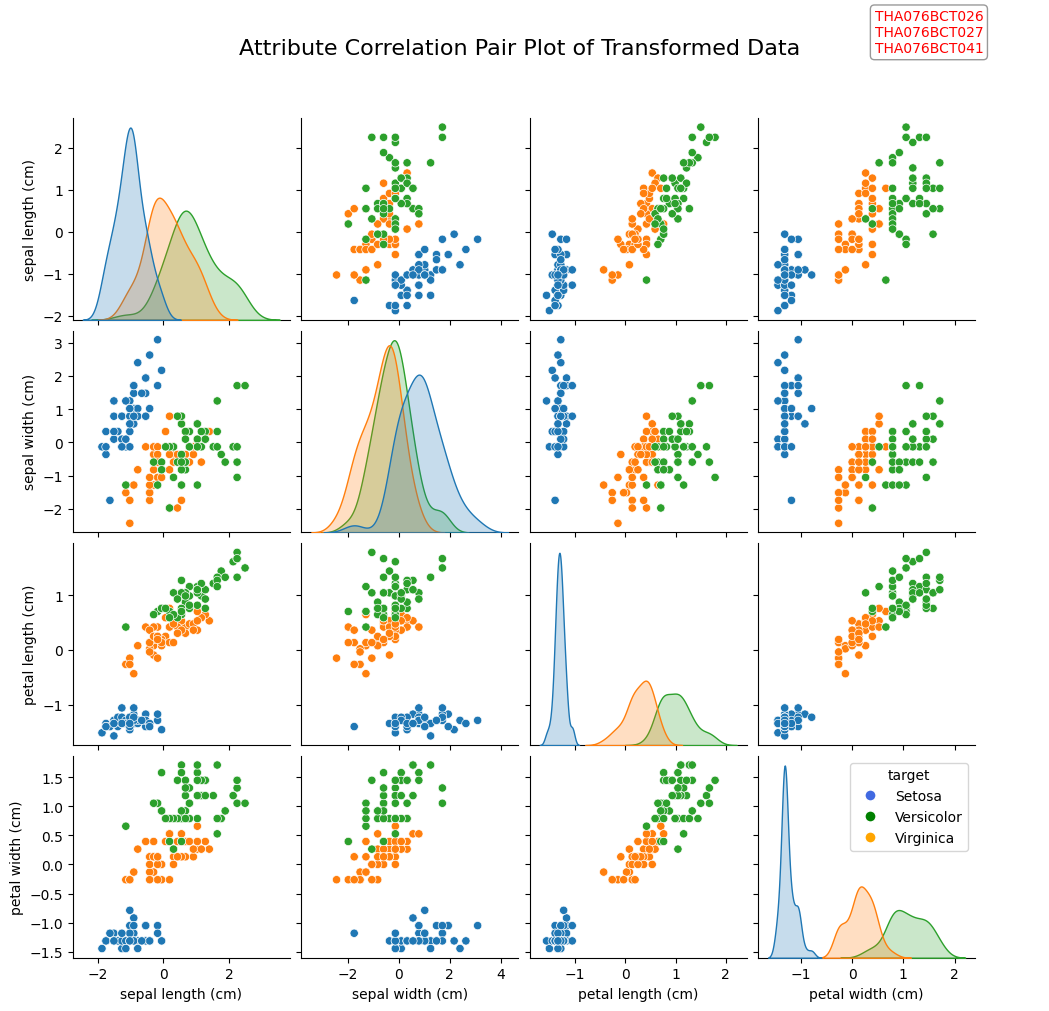
\includegraphics{PCA on IRIS_files/PCA on IRIS_17_1.png}
\caption{png}
\end{figure}

\begin{lstlisting}[language=Python]
# lets see the new plot after standardization
plt.figure(figsize=(10, 6))
plt.scatter(df_scaled['sepal length (cm)'], df_scaled['sepal width (cm)'], c=df_scaled['target'], label='Sepal')
plt.scatter(df_scaled['petal length (cm)'], df_scaled['petal width (cm)'], c=df_scaled['target'], marker='x', label='Petal')
plt.xlabel('Length (cm)')
plt.ylabel('Width (cm)')
plt.title('Scatter Plot of Sepal and Petal Features')
plt.colorbar(label='Species')
plt.ylim(-3,4)
plt.xlim(-3,3)
plt.text(-1, 3.5, "'THA076BCT026','THA076BCT027','THA076BCT041'", fontsize=8,color='red')

plt.legend()
plt.savefig('./plots/processed Sepal and Petal Feature', bbox_inches='tight')
plt.show()
\end{lstlisting}

\begin{figure}
\centering
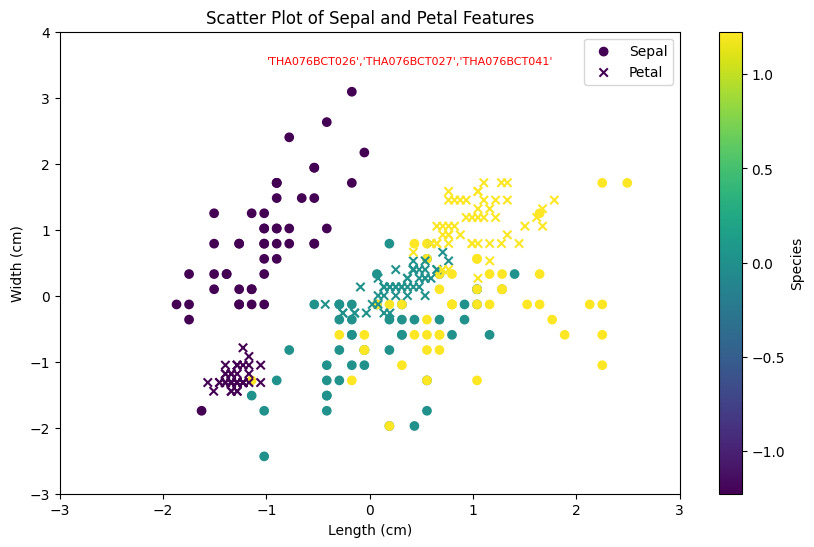
\includegraphics{PCA on IRIS_files/PCA on IRIS_18_0.png}
\caption{png}
\end{figure}

\textbf{STEP 4: Covariance matrix calculation.}

\begin{lstlisting}[language=Python]
# this cell is not necessary.
# X_train is already an array so no need to do data_matrix = np.array(X)
data_matrix = X_train
data_matrix.shape
\end{lstlisting}

\begin{lstlisting}
(150, 4)
\end{lstlisting}

\begin{lstlisting}[language=Python]
# covariance matrix will be 4*4 since x=(150,4)

covariance_matrix = np.cov(X_train, rowvar=False)             # row of X_train != variable(so column of X_train means variable, and rows means observation)
print("Covariance matrix shape:", covariance_matrix.shape)
print(covariance_matrix)
\end{lstlisting}

\begin{lstlisting}
Covariance matrix shape: (4, 4)
[[ 1.00671141 -0.11835884  0.87760447  0.82343066]
 [-0.11835884  1.00671141 -0.43131554 -0.36858315]
 [ 0.87760447 -0.43131554  1.00671141  0.96932762]
 [ 0.82343066 -0.36858315  0.96932762  1.00671141]]
\end{lstlisting}

\begin{lstlisting}[language=Python]
# visualize covariance matrix
plt.imshow(covariance_matrix, cmap='Blues', interpolation='nearest')
plt.colorbar()
plt.title('Covariance Matrix')

plt.text(0, -0.8, "'THA076BCT026','THA076BCT027','THA076BCT041'", fontsize=8,color='red')
plt.xticks(np.arange(4), np.arange(4))   #tick labels on axes changed from 0 to 4
plt.yticks(np.arange(4), np.arange(4))
plt.savefig('Iris Covariance Matrix', bbox_inches='tight')
plt.show()
\end{lstlisting}

\begin{figure}
\centering
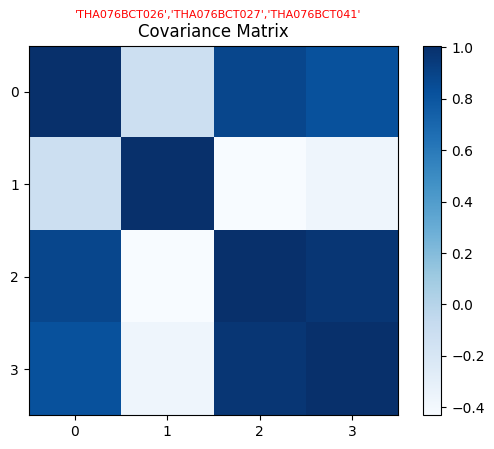
\includegraphics{PCA on IRIS_files/PCA on IRIS_22_0.png}
\caption{png}
\end{figure}

\textbf{STEP 5: Eigen values and eigen vector calculation}

\begin{lstlisting}[language=Python]
eigenvalues, eigenvectors = np.linalg.eig(covariance_matrix)
#descending sort
sorted_indices = np.argsort(eigenvalues)[::-1]
eigenvalues = eigenvalues[sorted_indices]
eigenvectors = eigenvectors[:, sorted_indices]

print("eigen values are",eigenvalues)
print("eigen vectors are",eigenvectors)
print(eigenvalues.shape)
print(eigenvectors.shape)
\end{lstlisting}

\begin{lstlisting}
eigen values are [2.93808505 0.9201649  0.14774182 0.02085386]
eigen vectors are [[ 0.52106591 -0.37741762 -0.71956635  0.26128628]
 [-0.26934744 -0.92329566  0.24438178 -0.12350962]
 [ 0.5804131  -0.02449161  0.14212637 -0.80144925]
 [ 0.56485654 -0.06694199  0.63427274  0.52359713]]
(4,)
(4, 4)
\end{lstlisting}

\textbf{STEP 6: See the variance explained by each eigen values.}

\begin{lstlisting}[language=Python]
# Proportion of variance for each eigen values
pov_list=[]
for i in range (0,4):
  pov=eigenvalues[i]/sum(eigenvalues)
  pov_list.append(pov)
  print("Proportion of variance for", eigenvalues[i],"eigen value is", pov)
\end{lstlisting}

\begin{lstlisting}
Proportion of variance for 2.9380850501999944 eigen value is 0.7296244541329987
Proportion of variance for 0.9201649041624874 eigen value is 0.22850761786701773
Proportion of variance for 0.14774182104494807 eigen value is 0.03668921889282877
Proportion of variance for 0.02085386217646228 eigen value is 0.0051787091071548
\end{lstlisting}

\begin{lstlisting}[language=Python]
# Plot the scree plot
plt.plot(range(1, len(pov_list) + 1), pov_list, marker='o',color='blue')
varlegend= "'THA076BCT026','THA076BCT027','THA076BCT041'"
plt.text(2.5,0.7,varlegend,color='red')   #plt.text(x_position, y_position, varlegend)
plt.xlabel('Principal Component')
plt.ylabel('Proportion of Variance')
plt.title('Scree Plot')
plt.show()
\end{lstlisting}

\begin{figure}
\centering
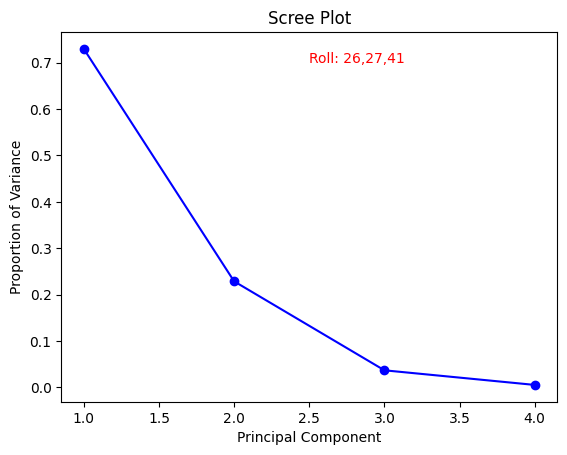
\includegraphics{PCA on IRIS_files/PCA on IRIS_27_0.png}
\caption{png}
\end{figure}

\textbf{STEP 7: Select the eigen vectors as needed to compute the final
output}

\begin{lstlisting}[language=Python]
print("Shape of x train is",X_train.shape)
transposed_X_train = np.transpose(X_train)
transposed_X_train.shape
\end{lstlisting}

\begin{lstlisting}
Shape of x train is (150, 4)





(4, 150)
\end{lstlisting}

\begin{lstlisting}[language=Python]
eigenvectors_transposed=np.transpose(eigenvectors)
\end{lstlisting}

\begin{lstlisting}[language=Python]
final_data = {}       # Dictionary to store the final projected data

# Define the combinations of selected components
selected_components = [[0], [0, 1], [0,2], [0, 3], [1], [1,2], [1,3], [0, 1, 2, 3]]
count=len(selected_components)

# Iterate over the selected components
for i in range (0,count):
  selected_eigenvectors = eigenvectors_transposed[selected_components[i]]              #select the combination of components from above list
  final_data[i] = np.transpose(selected_eigenvectors @ transposed_X_train)  #projection
  print(final_data[i].shape)
\end{lstlisting}

\begin{lstlisting}
(150, 1)
(150, 2)
(150, 2)
(150, 2)
(150, 1)
(150, 2)
(150, 2)
(150, 4)
\end{lstlisting}

\begin{lstlisting}[language=Python]
eigenvalues
\end{lstlisting}

\begin{lstlisting}
array([2.93808505, 0.9201649 , 0.14774182, 0.02085386])
\end{lstlisting}

\begin{lstlisting}[language=Python]
eigenvectors
\end{lstlisting}

\begin{lstlisting}
array([[ 0.52106591, -0.37741762, -0.71956635,  0.26128628],
       [-0.26934744, -0.92329566,  0.24438178, -0.12350962],
       [ 0.5804131 , -0.02449161,  0.14212637, -0.80144925],
       [ 0.56485654, -0.06694199,  0.63427274,  0.52359713]])
\end{lstlisting}

\begin{lstlisting}[language=Python]
eigenvectors_transposed[selected_components[2]]
\end{lstlisting}

\begin{lstlisting}
array([[ 0.52106591, -0.26934744,  0.5804131 ,  0.56485654],
       [-0.71956635,  0.24438178,  0.14212637,  0.63427274]])
\end{lstlisting}

\textbf{STEP 8: Computing and visualizing covariance for the new data.}

\begin{lstlisting}[language=Python]
new_covariance_matrices_dictionary = {}
# Compute covariance matrix for each projected data
for i in range(0, count):
    print(" * Covariance matrix for combination no", i)
    new_covariance_matrix = np.cov(final_data[i], rowvar=False)
    new_covariance_matrices_dictionary[i] = new_covariance_matrix
    # Print the shape of the covariance matrix
    print("  --->Covariance matrix shape:", new_covariance_matrix.shape)
\end{lstlisting}

\begin{lstlisting}
 * Covariance matrix for combination no 0
  --->Covariance matrix shape: ()
 * Covariance matrix for combination no 1
  --->Covariance matrix shape: (2, 2)
 * Covariance matrix for combination no 2
  --->Covariance matrix shape: (2, 2)
 * Covariance matrix for combination no 3
  --->Covariance matrix shape: (2, 2)
 * Covariance matrix for combination no 4
  --->Covariance matrix shape: ()
 * Covariance matrix for combination no 5
  --->Covariance matrix shape: (2, 2)
 * Covariance matrix for combination no 6
  --->Covariance matrix shape: (2, 2)
 * Covariance matrix for combination no 7
  --->Covariance matrix shape: (4, 4)
\end{lstlisting}

\begin{lstlisting}[language=Python]
#Lets access the first combination(combination 0), which is (eigen[0])                    (best component)
new_covariance_matrices_dictionary[0]
\end{lstlisting}

\begin{lstlisting}
array(2.93808505)
\end{lstlisting}

\begin{lstlisting}[language=Python]
#Lets access combination 1, which is eigen[0] and eigen[1]              (2 best components)
new_covariance_matrices_dictionary[1]
\end{lstlisting}

\begin{lstlisting}
array([[2.93808505e+00, 2.86124592e-16],
       [2.86124592e-16, 9.20164904e-01]])
\end{lstlisting}

\begin{lstlisting}[language=Python]
#Lets access combination 3, which is eigen[0] and eigen[3]           (best and worst component)
new_covariance_matrices_dictionary[3]
\end{lstlisting}

\begin{lstlisting}
array([[ 2.93808505e+00, -2.74202734e-16],
       [-2.74202734e-16,  2.08538622e-02]])
\end{lstlisting}

\begin{lstlisting}[language=Python]
#Lets access combination 5, which is eigen[1] and eigen[2]        (2 medium medium best components)
new_covariance_matrices_dictionary[5]
\end{lstlisting}

\begin{lstlisting}
array([[ 9.20164904e-01, -4.78783679e-16],
       [-4.78783679e-16,  1.47741821e-01]])
\end{lstlisting}

\begin{lstlisting}[language=Python]
#Lets access combination 7, which is eigen[0],eigen[1],eigen[2] and eigen[3]      (all components combined)
new_covariance_matrices_dictionary[7]
\end{lstlisting}

\begin{lstlisting}
array([[ 2.93808505e+00,  2.86124592e-16,  2.47378553e-16,
        -2.74202734e-16],
       [ 2.86124592e-16,  9.20164904e-01, -4.78783679e-16,
         3.12948772e-17],
       [ 2.47378553e-16, -4.78783679e-16,  1.47741821e-01,
         5.06678964e-17],
       [-2.74202734e-16,  3.12948772e-17,  5.06678964e-17,
         2.08538622e-02]])
\end{lstlisting}

\begin{lstlisting}[language=Python]
# Heatmap plot, darker shade indicate higher values. (combination starts from 0 to 7)
plt.imshow(new_covariance_matrices_dictionary[1], cmap='Reds', interpolation='nearest')  #for smoother interpolation of color on pixel values, instead of 'nearest', we can use 'bilinear','bicubic','spline16', 'spline36', 'hanning', 'hamming', 'hermite',etc..
plt.colorbar()
plt.title("New Covariance Matrix Combination 1 (2 best PC)")
plt.text(-0.3, -0.66, "'THA076BCT026','THA076BCT027','THA076BCT041'", fontsize=8,color='red')
plt.savefig('Covariance Matrix for 2 best PC', bbox_inches='tight')
plt.show()
\end{lstlisting}

\begin{figure}
\centering
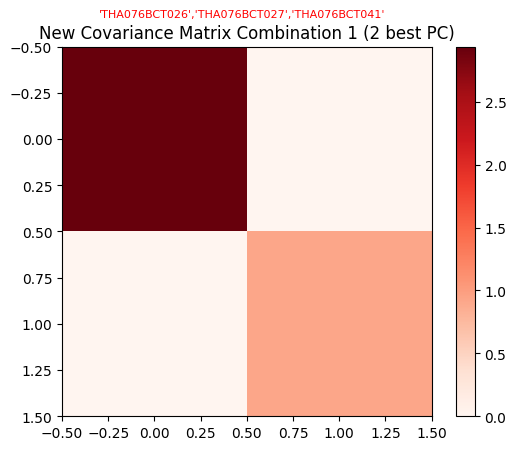
\includegraphics{PCA on IRIS_files/PCA on IRIS_42_0.png}
\caption{png}
\end{figure}

\begin{lstlisting}[language=Python]
plt.imshow(new_covariance_matrices_dictionary[3], cmap='Reds', interpolation='nearest')
plt.colorbar()
plt.title("New Covariance Matrix Combination 3 (best and worst PC)")
plt.text(-0.3, -0.66, "'THA076BCT026','THA076BCT027','THA076BCT041'", fontsize=8,color='red')
plt.savefig('Covariance Matrix for best and worst PC', bbox_inches='tight')
plt.show()
\end{lstlisting}

\begin{figure}
\centering
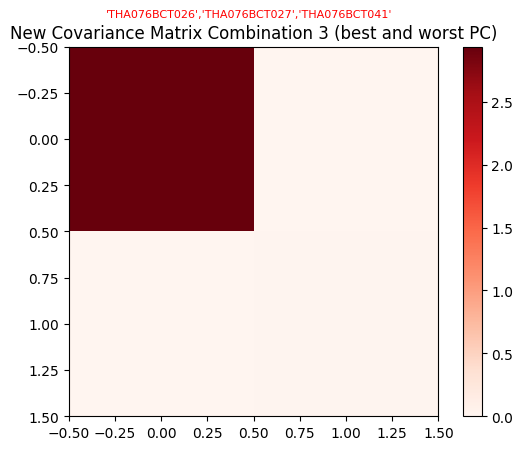
\includegraphics{PCA on IRIS_files/PCA on IRIS_43_0.png}
\caption{png}
\end{figure}

\begin{lstlisting}[language=Python]
plt.imshow(new_covariance_matrices_dictionary[5], cmap='Reds', interpolation='nearest')
plt.colorbar()
plt.title("Covariance Matrix for two medium PCs")
plt.text(-0.3, -0.66, "'THA076BCT026','THA076BCT027','THA076BCT041'", fontsize=8,color='red')
plt.savefig('Covariance Matrix for two medium PCs', bbox_inches='tight')
plt.show()
\end{lstlisting}

\begin{figure}
\centering
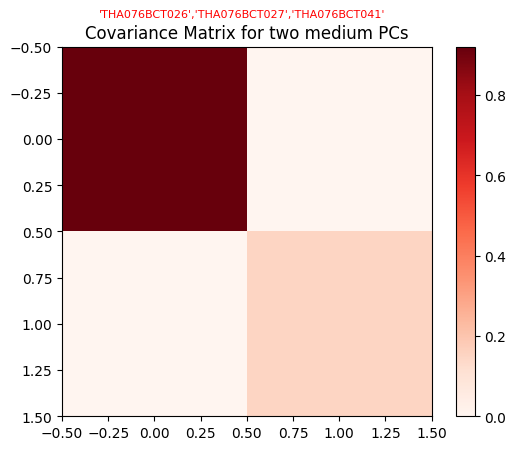
\includegraphics{PCA on IRIS_files/PCA on IRIS_44_0.png}
\caption{png}
\end{figure}

\begin{lstlisting}[language=Python]
plt.imshow(new_covariance_matrices_dictionary[7], cmap='Reds', interpolation='nearest')
plt.colorbar()
plt.title("New Covariance Matrix Combination 7 (All Components)")
plt.show()
\end{lstlisting}

\begin{figure}
\centering
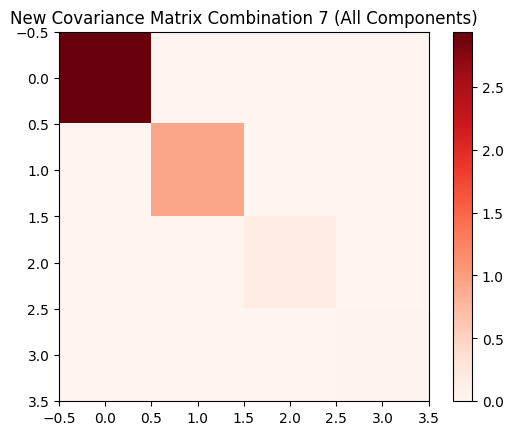
\includegraphics{PCA on IRIS_files/PCA on IRIS_45_0.png}
\caption{png}
\end{figure}

\textbf{STEP 9: Obtain final data and visualize}

\begin{lstlisting}[language=Python]
# Two best PCs
final_data[1].shape
#final_data[1]
\end{lstlisting}

\begin{lstlisting}
(150, 2)
\end{lstlisting}

\begin{lstlisting}[language=Python]
plt.ylim(-3,3)
plt.xlim(-3,3)
# plt.title("2 best PCs")
plt.xlabel('PC1')
plt.ylabel('PC2')
plt.title("Scatter Plot after PCA for two best PCs on IRIS Dataset")
plt.text(-1.8, 2.8, "'THA076BCT026','THA076BCT027','THA076BCT041'", fontsize=8,color='red')
plt.scatter(final_data[1][:,0],final_data[1][:,1],c=y)
plt.savefig('Scatter Plot after PCA for two best PCs', bbox_inches='tight')
\end{lstlisting}

\begin{figure}
\centering
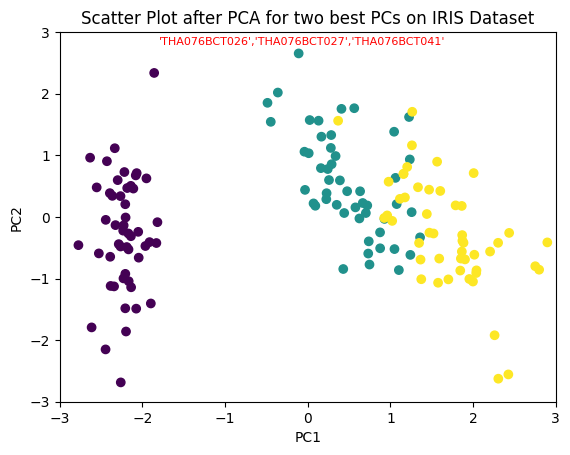
\includegraphics{PCA on IRIS_files/PCA on IRIS_48_0.png}
\caption{png}
\end{figure}

\begin{lstlisting}[language=Python]
#Best and worst PCs
final_data[3].shape
#final_data[3]
\end{lstlisting}

\begin{lstlisting}
(150, 2)
\end{lstlisting}

\begin{lstlisting}[language=Python]
plt.ylim(-3,3)
plt.xlim(-3,3)
plt.xlabel('PC1')
plt.ylabel('PC4')
plt.title("Scatter Plot after PCA for Best and worst PCs on IRIS Dataset")
plt.text(-1.8, 2.8, "'THA076BCT026','THA076BCT027','THA076BCT041'", fontsize=8,color='red')
plt.scatter(final_data[3][:,0],final_data[3][:,1],c=y)
plt.savefig('Scatter Plot after PCA for Best and worst PCs', bbox_inches='tight')
\end{lstlisting}

\begin{figure}
\centering
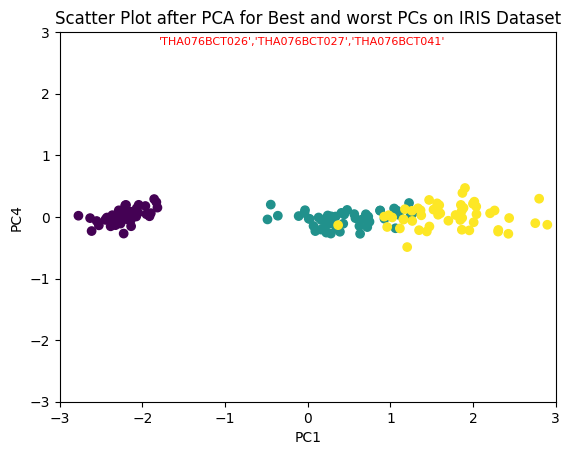
\includegraphics{PCA on IRIS_files/PCA on IRIS_50_0.png}
\caption{png}
\end{figure}

\begin{lstlisting}[language=Python]
#Best and mediumly worse PCs
final_data[5].shape
#final_data[5]
\end{lstlisting}

\begin{lstlisting}
(150, 2)
\end{lstlisting}

\begin{lstlisting}[language=Python]
plt.ylim(-3,3)
plt.xlim(-3,3)
plt.title("Scatter Plot after PCA for two Medium PCs on IRIS Dataset")
plt.text(-1.8, 2.8, "'THA076BCT026','THA076BCT027','THA076BCT041'", fontsize=8,color='red')
plt.xlabel('PC2')
plt.ylabel('PC3')
plt.scatter(final_data[5][:,0],final_data[5][:,1],c=y)
plt.savefig('Scatter Plot after PCA for two Medium PCs', bbox_inches='tight')
\end{lstlisting}

\begin{figure}
\centering
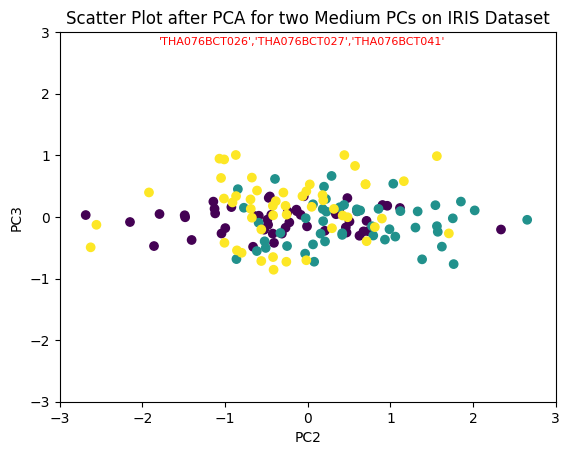
\includegraphics{PCA on IRIS_files/PCA on IRIS_52_0.png}
\caption{png}
\end{figure}

\begin{lstlisting}[language=Python]
#All components
final_data[7].shape
#final_data[7]
\end{lstlisting}

\begin{lstlisting}
(150, 4)
\end{lstlisting}

\begin{lstlisting}[language=Python]
plt.ylim(-3,3)
plt.xlim(-3,3)
plt.title("All PCs")
plt.xlabel('PC1')
plt.ylabel('PC2')
plt.scatter(final_data[7][:,0],final_data[7][:,1],c=y)
\end{lstlisting}

\begin{lstlisting}
<matplotlib.collections.PathCollection at 0x14c5f056ee0>
\end{lstlisting}

\begin{figure}
\centering
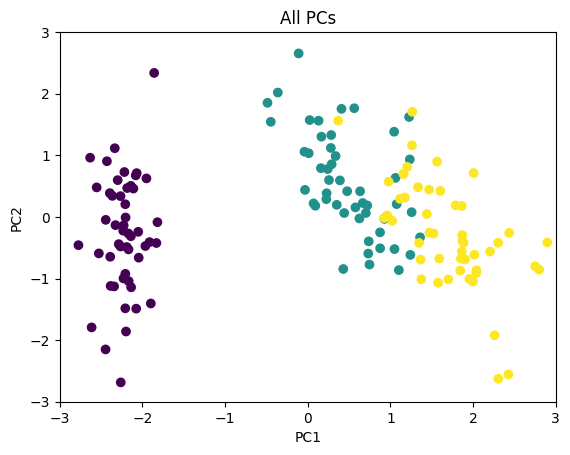
\includegraphics{PCA on IRIS_files/PCA on IRIS_54_1.png}
\caption{png}
\end{figure}

\begin{lstlisting}[language=Python]
# Create a 3D scatter plot
from mpl_toolkits.mplot3d import Axes3D

fig = plt.figure()
fig = plt.figure(figsize=(8, 8))
ax = fig.add_subplot(111, projection='3d')
ax.scatter(final_data[7][:,0],final_data[7][:,1],final_data[7][:,2],c=y, marker='o')
ax.set_xlabel('PC1')
ax.set_ylabel('PC2')
ax.set_zlabel('PC3')
ax.set_title('3D Scatter Plot of 3 PCs')
ax.text(-6, 2.8,1, "'THA076BCT026','THA076BCT027','THA076BCT041'", fontsize=8,color='red')
plt.tight_layout()
plt.savefig('3D Scatter Plot of 3 PCs', bbox_inches='tight',dpi=300)
plt.show()
\end{lstlisting}

\begin{lstlisting}
<Figure size 640x480 with 0 Axes>
\end{lstlisting}

\begin{figure}
\centering
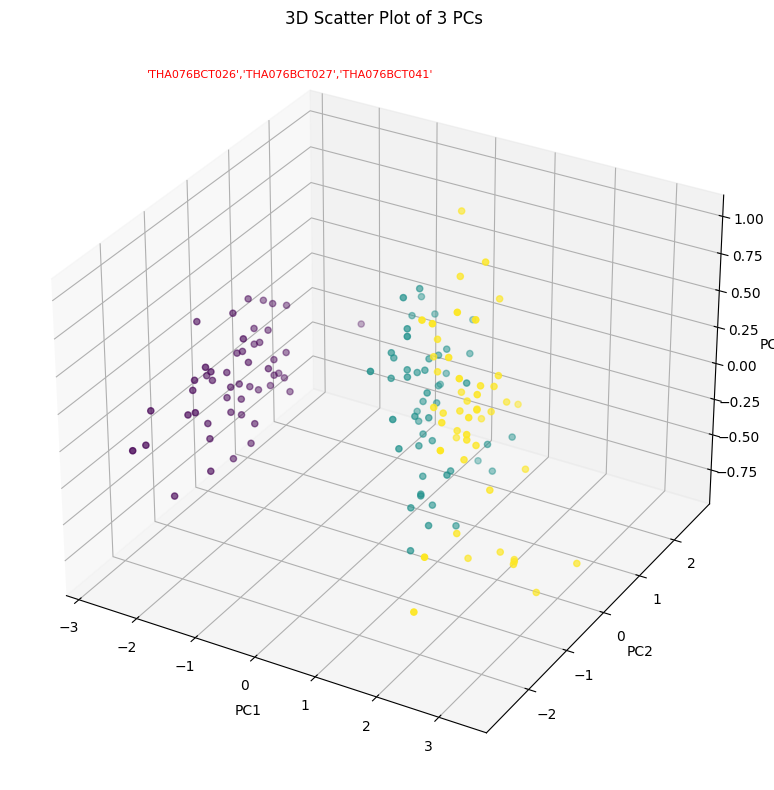
\includegraphics{PCA on IRIS_files/PCA on IRIS_55_1.png}
\caption{png}
\end{figure}

\textbf{STEP 10: PCA with library.}

\begin{lstlisting}[language=Python]
from sklearn.decomposition import PCA
# Create instances of PCA with the desired number of components. (pca1 = 2components. pca2=so as to retain 95% info)
pca1 = PCA(n_components=2)
pca2 = PCA(0.95)

# Fit the PCA model to the data and transform the data
reduced_data1 = pca1.fit_transform(X)
reduced_data2 = pca2.fit_transform(X)

# Print the shape of the reduced data
print("Shape of reduced data:", reduced_data1.shape)
print("reduced through first",reduced_data1)

print("Shape of reduced data:", reduced_data2.shape)
print("reduced through second",reduced_data2)
\end{lstlisting}

\textbf{STEP 11: Lets train 4 models and visualize the results.} 2
models are implemented after applying PCA using library. The third model
is implemented after applying PCA using Math(using all the earlier above
steps). The fourth model is trained without PCA.

\begin{lstlisting}[language=Python]
# Create 4 sets of test-train for 4 models.
from sklearn.model_selection import train_test_split
x_train1,x_test1,y_train1,y_test1 = train_test_split(reduced_data1,y,test_size=0.2)   # using library, 2 components
x_train2,x_test2,y_train2,y_test2 = train_test_split(reduced_data2,y,test_size=0.2)   # using library, 0.95 info
x_train3,x_test3,y_train3,y_test3 = train_test_split(final_data[1],y,test_size=0.2)   # from scratch, 2 components
x_train4,x_test4,y_train4,y_test4 = train_test_split(X_train,y,test_size=0.2)         # no PCA
\end{lstlisting}

\begin{lstlisting}[language=Python]
#training of the model
# model 1: using library, 2 components
from sklearn.svm import SVC
svm1 = SVC()
svm1.fit(x_train1, y_train1)
\end{lstlisting}

\hypertarget{sk-container-id-33}{}
In a Jupyter environment, please rerun this cell to show the HTML
representation or trust the notebook. On GitHub, the HTML representation
is unable to render, please try loading this page with nbviewer.org.

SVC

\begin{lstlisting}[language=Python]
#library, 0.95 info
svm2=SVC()
svm2.fit(x_train2, y_train2)
\end{lstlisting}

\hypertarget{sk-container-id-34}{}
In a Jupyter environment, please rerun this cell to show the HTML
representation or trust the notebook. On GitHub, the HTML representation
is unable to render, please try loading this page with nbviewer.org.

SVC

\begin{lstlisting}[language=Python]
#from scratch, 2 components
svm3=SVC()
svm3.fit(x_train3, y_train3)
\end{lstlisting}

\hypertarget{sk-container-id-35}{}
In a Jupyter environment, please rerun this cell to show the HTML
representation or trust the notebook. On GitHub, the HTML representation
is unable to render, please try loading this page with nbviewer.org.

SVC

\begin{lstlisting}[language=Python]
#No PCA
svm4=SVC()
svm4.fit(x_train4, y_train4)
\end{lstlisting}

\hypertarget{sk-container-id-36}{}
In a Jupyter environment, please rerun this cell to show the HTML
representation or trust the notebook. On GitHub, the HTML representation
is unable to render, please try loading this page with nbviewer.org.

SVC

\begin{lstlisting}[language=Python]
# Accuracy check for 4 models
from sklearn.metrics import accuracy_score

y_pred1 = svm1.predict(x_test1)
accuracy1 = accuracy_score(y_test1, y_pred1)
print("Accuracy1:", accuracy1)

y_pred2 = svm2.predict(x_test2)
accuracy2 = accuracy_score(y_test2, y_pred2)
print("Accuracy2:", accuracy2)

y_pred3 = svm3.predict(x_test3)
accuracy3 = accuracy_score(y_test3, y_pred3)
print("Accuracy3:", accuracy3)

y_pred4 = svm4.predict(x_test4)
accuracy4 = accuracy_score(y_test4, y_pred4)
print("Accuracy4:", accuracy4)
\end{lstlisting}

\begin{lstlisting}
Accuracy1: 0.9666666666666667
Accuracy2: 0.9333333333333333
Accuracy3: 0.9666666666666667
Accuracy4: 0.9666666666666667
\end{lstlisting}

\begin{lstlisting}[language=Python]
#prediciton from 4 models
predictions1 = svm1.predict(x_test1)
predictions2 = svm2.predict(x_test2)
predictions3 = svm3.predict(x_test3)
predictions4 = svm4.predict(x_test4)
predictions1.shape
\end{lstlisting}

\begin{lstlisting}
(30,)
\end{lstlisting}

\begin{lstlisting}[language=Python]
# Lets define a function to plot confusion matrix
from sklearn.metrics import confusion_matrix
import seaborn as sns
def plot_confusion_matrix(y_true, y_pred, model_name,text):
    cm = confusion_matrix(y_true, y_pred)
    sns.heatmap(cm, annot=True, cmap="Blues", fmt="d")
    plt.title(f"Confusion Matrix - {model_name}")
    plt.xlabel("Predicted Labels")
    plt.ylabel("True Labels")
    plt.text(0.2, -0.5, "'THA076BCT026','THA076BCT027','THA076BCT041'", fontsize=8,color='red')
    plt.savefig(f'./plots/{model_name}.png', bbox_inches='tight',dpi=300)
    plt.show()
\end{lstlisting}

\begin{lstlisting}[language=Python]
# Plot confusion matrix for model 1
plot_confusion_matrix(y_test1, predictions1, "UsingLibrary, 2 Components")
\end{lstlisting}

\begin{figure}
\centering
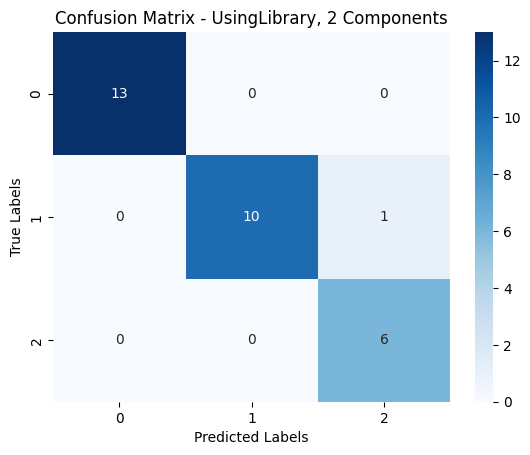
\includegraphics{PCA on IRIS_files/PCA on IRIS_67_0.png}
\caption{png}
\end{figure}

\begin{lstlisting}[language=Python]
# for model 2
plot_confusion_matrix(y_test2, predictions2, "Using Library, 0.95 Info retention")
\end{lstlisting}

\begin{figure}
\centering
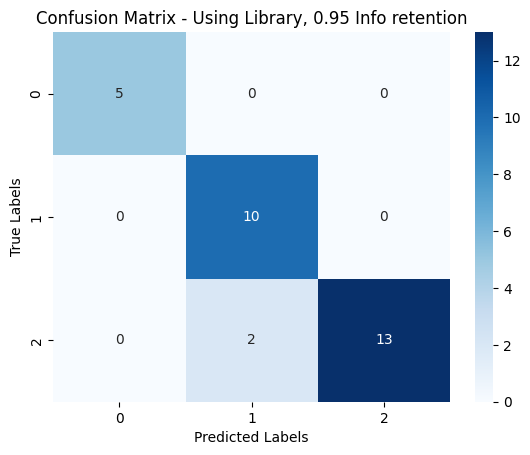
\includegraphics{PCA on IRIS_files/PCA on IRIS_68_0.png}
\caption{png}
\end{figure}

\begin{lstlisting}[language=Python]
#for model 3
plot_confusion_matrix(y_test3, predictions3, "From Scratch, 2 Components")
\end{lstlisting}

\begin{figure}
\centering
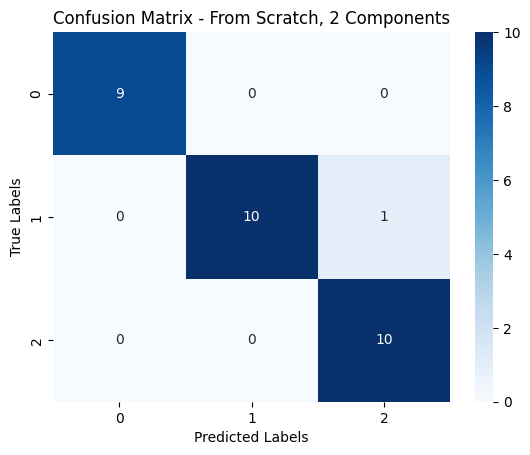
\includegraphics{PCA on IRIS_files/PCA on IRIS_69_0.png}
\caption{png}
\end{figure}

\begin{lstlisting}[language=Python]
#for model4
plot_confusion_matrix(y_test4, predictions4, "No PCA")
\end{lstlisting}

\begin{figure}
\centering
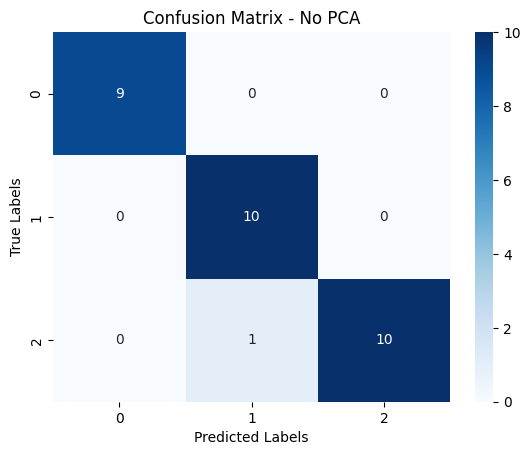
\includegraphics{PCA on IRIS_files/PCA on IRIS_70_0.png}
\caption{png}
\end{figure}

\end{document}
